\documentclass[a4paper,12pt,twocolumn]{article}
\usepackage{tabularx} % extra features for tabular environment
\usepackage{amsmath}  % improve math presentation
\usepackage{graphicx} % takes care of graphic including machinery
\usepackage[margin=1in,letterpaper]{geometry} % decreases margins
\usepackage{cite} % takes care of citations
\usepackage[final]{hyperref} % adds hyper links inside the generated pdf file
\usepackage{booktabs,caption}
\usepackage{threeparttable}
\usepackage{graphicx} 
\usepackage{float}
\hypersetup{
	colorlinks=true,       % false: boxed links; true: colored links
	linkcolor=black,        % color of internal links
	citecolor=black,        % color of links to bibliography
	filecolor=magenta,     % color of file links
	urlcolor=black         
}

\begin{document}

\begin{titlepage}
	\begin{center}
		
		\thispagestyle{empty}
		
		\Huge{
			\textbf{UCD School Of Physics}
		}
		
		\vspace{1cm}	
		
		
\includegraphics[scale=0.08]{UCDLogo.png}
		
		\vspace{1cm}
		
		\large{
			\textbf{PHYC30170 Physics with Astronomy and Space Science Lab 1; \\
				Frequency Dependence of the Skin Depth in a Metal Cylinder \\
				\vspace{1cm}
				22/09/2022 \\
				\vspace{1cm}
				Daragh Hollman}
		} \\
		
	\end{center}
\end{titlepage}

\twocolumn[
\begin{@twocolumnfalse}
	\begin{abstract}
		...
	\end{abstract}
\end{@twocolumnfalse}
]

\section{Introduction}
	Lorem ipsum dolor sit amet, consectetur adipiscing elit. Nulla semper ipsum laoreet accumsan malesuada. Proin quis metus justo. Quisque cursus posuere nisi eu sodales. Ut eu convallis nisi. Aliquam euismod maximus libero, at suscipit libero egestas faucibus. Sed egestas mi et enim sollicitudin, sed molestie erat consequat. Integer vel ex in nisl rhoncus laoreet vel viverra sapien. Vestibulum aliquet convallis leo, quis ultrices mi mollis ac. Aliquam vel lectus sit amet dolor eleifend dictum in mattis dolor. Nunc nunc odio, tristique id rutrum quis, lacinia in purus. Quisque vitae vestibulum magna.
	
\section{Theory}
	Present key equations without deriving.
	
	Vestibulum luctus massa leo, vitae commodo purus aliquet a. Maecenas arcu urna, vehicula et posuere ac, vestibulum eget dui. Integer vel dignissim augue, eu tristique urna. Nulla eget risus et nisi feugiat ornare eu ac elit. Etiam non hendrerit leo, at sollicitudin nulla. Phasellus molestie massa in diam ultricies elementum. Class aptent taciti sociosqu ad litora torquent per conubia nostra, per inceptos himenaeos. Etiam sed felis fringilla, rhoncus augue aliquam, mattis magna. Phasellus tincidunt blandit arcu, vitae egestas quam convallis vitae.
	
	Nam facilisis nibh in libero pharetra lacinia convallis vitae velit. Donec consectetur sed erat ac eleifend. Nunc ac sapien mauris. Maecenas at facilisis urna. Fusce commodo ultricies massa et porttitor. In venenatis aliquet nibh id fermentum. Sed libero sem, fringilla nec placerat sed, iaculis a mauris. Nullam aliquet interdum finibus. Nam ante metus, aliquam nec aliquam ut, ullamcorper eget lacus. Maecenas sed mauris ut tellus congue vulputate nec at tortor. Vivamus facilisis ornare facilisis. Pellentesque venenatis elit et lacus rhoncus viverra.
	
\section{Methodology}
	
	\begin{figure}
		\centering
		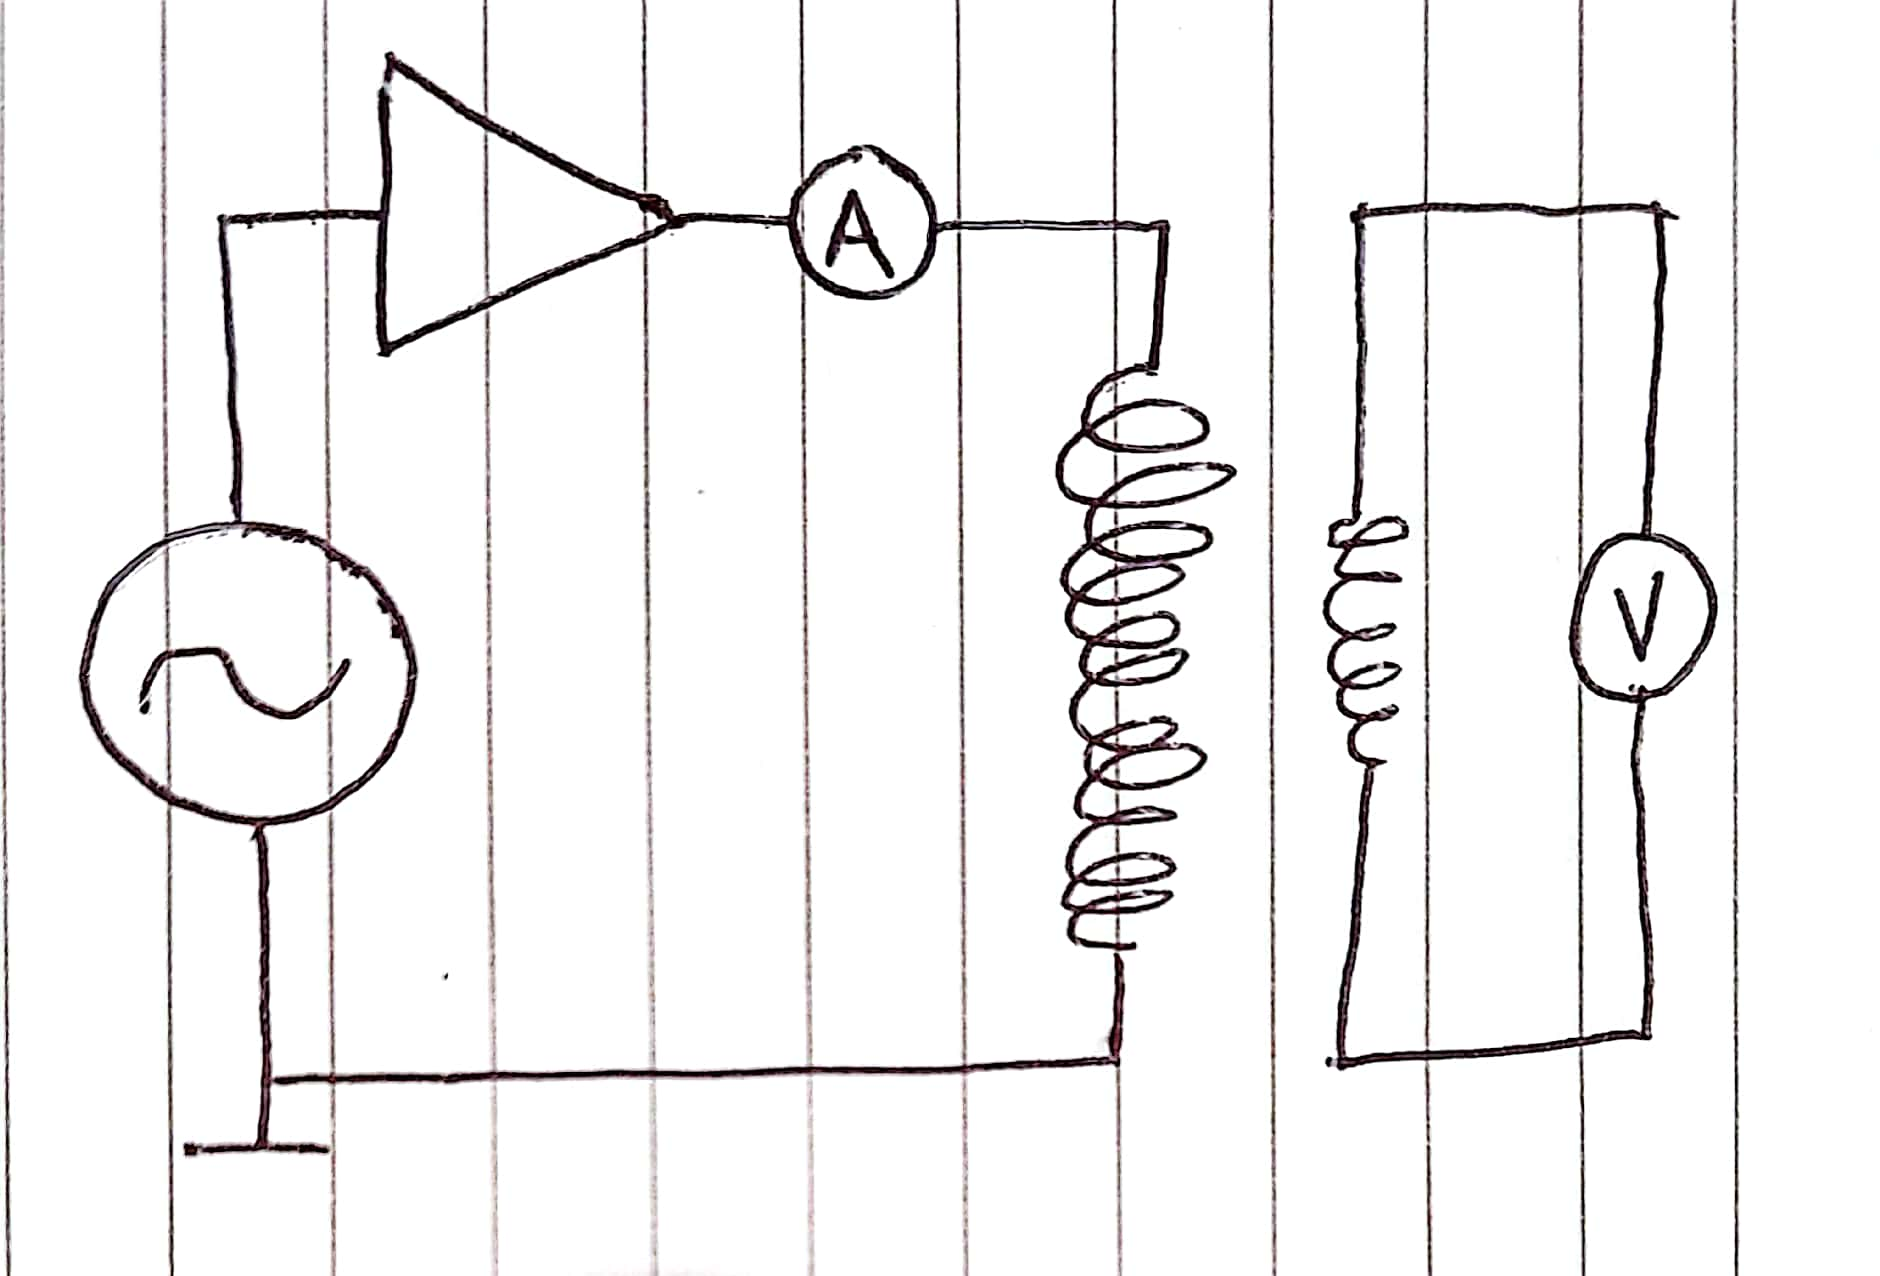
\includegraphics[scale=0.1]{SDcircuit.jpg}
		\captionsetup{font=scriptsize}
		\caption{Circuit diagram of the skin depth apparatus}
		\label{fig:circuit}
	\end{figure}

	\begin{figure}
		\centering
		\includegraphics[scale=0.045]{SDPhoto.jpg}
		\captionsetup{font=scriptsize}
		\caption{Photo of the skin depth apparatus, the metal cylinders were held inside the primary coil and  }
		\label{fig:photo}
	\end{figure}

	The apparatus was setup as shown in figures \ref{fig:circuit} and \ref{fig:photo}. The induction field was created by a solenoid of length $L_1 = (389 \pm 0.5) \,\text{mm}$ which contained $N_1 = 900 \pm $ turns of an insulated copper wire wound on a hollow tube - which the metal cylinders were inserted into. The signal to this solenoid was created by an AC signal generator and amplified. The rms current was kept constant at $I = (19 \pm 0.1)\,\text{mA}$. Although the accuracy of the ammeter used was higher, a larger uncertainty was used in practice to account for the very high sensitivity of adjusting the amplitude of the signal generator's output.
	
\section{Results and Analysis}
	Aliquam risus tortor, pharetra non suscipit ut, dictum in eros. In hac habitasse platea dictumst. Aenean lacinia sit amet ante vulputate mollis. Morbi non pulvinar lectus. Nam dignissim lacinia dolor, non congue risus dignissim ac. Nam eget libero quis enim facilisis tempor. Proin tempus arcu nunc, vel maximus quam ultricies eget. Proin nec vehicula dui. Proin elementum, ex vel lacinia pellentesque, mauris ex vestibulum nunc, ut sollicitudin ante justo at sem. Maecenas venenatis maximus efficitur. In tempor interdum lacus, non pretium dolor aliquam sed. Nam auctor sed ex quis finibus. Nam sed maximus lorem, eu ullamcorper massa. Vestibulum ante ipsum primis in faucibus orci luctus et ultrices posuere cubilia curae;
	
	

\section{Conclusion}
	Vestibulum non facilisis sem. Quisque gravida accumsan nunc tincidunt molestie. Donec pharetra urna ut nunc ullamcorper, in tincidunt sem dignissim. Ut mattis leo eu erat elementum, id fermentum tortor sollicitudin. Vestibulum id erat in mauris aliquam vulputate non id augue. Mauris tincidunt ornare imperdiet. Aliquam tristique bibendum metus, dignissim pharetra lorem lacinia nec. Class aptent taciti sociosqu ad litora torquent per conubia nostra, per inceptos himenaeos. Maecenas sit amet pharetra leo. Morbi id hendrerit nulla. Nunc sit amet ligula risus. Mauris sed odio egestas, luctus odio at, ultricies tortor. Pellentesque semper enim vitae malesuada tempor. Aliquam at risus nisl. Curabitur venenatis, est eget hendrerit iaculis, nulla leo aliquam est, at commodo tellus arcu non eros. Nullam quis ipsum non urna porta sollicitudin.

\newpage
\begin{thebibliography}{}
	
	
\end{thebibliography}

	

\newpage

\section*{Appendices}
	
	
\end{document}
